\documentclass[t,14pt,aspectratio=169,usenames,dvipsnames,table]{beamer}
%%%%%%%%%%%%%%%%%%%%%%%%%%%%%%%%%%%%%%%%%%%%%%%%%%%%%%%%%%%%%%%%%%%%%%%%%%%%%%%%%%%%%%%
% To Pass graphics paths
%%%%%%%%%%%%%%%%%%%%%%%%%%%%%%%%%%%%%%%%%%%%%%%%%%%%%%%%%%%%%%%%%%%%%%%%%%%%%%%%%%%%%%%

\graphicspath{{./Figures/}}
\graphicspath{{./Figures/chapter-01/}}
%%%%%%%%%%%%%%%%%%%%%%%%%%%%%%%%%%%%%%%%%%%%%%%%%%%%%%%%%%%%%%%%%%%%%%%%%%%%%%%%%%%%%%%
% Packages Definition
%%%%%%%%%%%%%%%%%%%%%%%%%%%%%%%%%%%%%%%%%%%%%%%%%%%%%%%%%%%%%%%%%%%%%%%%%%%%%%%%%%%%%%%
%\input{preamble/ch_01_theme}
%\usepackage{preamble/dbt}
\usetheme[showmaxslides]{pureminimalistic}
%\usetheme[darkmode, showmaxslides]{pureminimalistic}





\newcommand{\code}[1]{\mbox{\color{yellow}{\texttt{\textbf{\normalsize #1}}}}}
\usepackage[toc,page]{appendix}
\usepackage{listings}
\usepackage{hyperref}
\usepackage{pgf,pgfpages}
\usepackage{graphicx}
\usepackage{units}
\usepackage[utf8]{inputenc}
\usepackage{multicol}
\usepackage{xspace}
\usepackage[utf8]{inputenc}
\usepackage{textcomp}% for '\textdegree' macro
\usepackage{utopia} %font utopia imported
\usepackage{fontawesome5}
\usepackage[center]{caption}
\usepackage{subcaption}
\usepackage{gensymb}
\usepackage{adjustbox}
\usepackage{marginnote}
\usepackage{makecell}
\usepackage{textpos}
\usepackage[default]{lato}
\usepackage[font=small,skip=0pt]{caption}
\usepackage{xcolor,colortbl}
\usepackage{import}
\usepackage{marvosym}
\usepackage{ulem} %Strikethrough
\usepackage[inkscapelatex=false]{svg}


%\overfullrule=2cm
%%%%%%%%%%%%%%%%%%%%%%%%%%%%%%%%%%%%%%%%%%%%%%%%%%%%%%%%%%%%%%%%%%%%%%%%%%%%%%%%%%%%%%%
\input{preamble/preamble_quote_custom_commands.tex}
%%%%%%%%%%%%%%%%%%%%%%%%%%%%%%%%%%%%%%%%%%%%%%%%%%%%%%%%%%%%%%%%%%%%%%%%%%%%%%%%%%%%%%%
\input{preamble/preamble_custom_commands.tex}
%%%%%%%%%%%%%%%%%%%%%%%%%%%%%%%%%%%%%%%%%%%%%%%%%%%%%%%%%%%%%%%%%%%%%%%%%%%%%%%%%%%%%%%
\input{preamble/tikz_preamble.tex}
%%%%%%%%%%%%%%%%%%%%%%%%%%%%%%%%%%%%%%%%%%%%%%%%%%%%%%%%%%%%%%%%%%%%%%%%%%%%%%%%%%%%%%%
%%%%%%%%%%%%%%%%%%%%%%%%%%%%%%%%%%%%%%%%%%%%%%%%%%%%%%%%%%%%%%%%%%%%%%%%%%%%%%%%%%%%%%%% 
%To define Code Syntax Scala
%%%%%%%%%%%%%%%%%%%%%%%%%%%%%%%%%%%%%%%%%%%%%%%%%%%%%%%%%%%%%%%%%%%%%%%%%%%%%%%%%%%%%%%% 
% Scala
%%%%%%%%%%%%%%%%%%%%%%%%%%%%%%%%%%%%%%%%%%%%%%%%%%%%%%%%%%%%%%%%%%%%%%%%%%%%%%%%%%%%%%%% 
\definecolor{mymauve}{rgb}{0.58,0,0.82}
\definecolor{dkgreen}{rgb}{0,0.6,0}
\definecolor{ltgray}{rgb}{0.5,0.5,0.5}
\usepackage{caption} % Add the caption package

% Redefine the lstlisting format to remove the unwanted prefix
\DeclareCaptionFormat{mylst}{#1#2#3}
\DeclareCaptionFont{mycolor}{\color{red}}
\renewcommand\lstlistingname{Code Snippet:}
\renewcommand\lstlistlistingname{Code Snippet:}
%\DeclareCaptionStyle{listing} [justification=raggedright,indention=0pt, labelfont=bf]{}
%\captionsetup[lstlisting]{style=listing, labelsep=none}

\captionsetup[lstlisting]{format=mylst,labelfont={color=harvardcrimson},labelsep=space,justification=raggedright}

\lstset{%
	frame=tb,
	language=scala,
	aboveskip=3mm,
	belowskip=3mm,
	showstringspaces=false,
	columns=flexible,
	numbers=left,                   % where to put the line-numbers
	numberstyle=\tiny\color{gray},  % the style that is used for the line-numbers
	stepnumber=1,                   % the step between two line-numbers. If it's 1, each line will be numbered
	numbersep=5pt,                  % how far the line-numbers are from the code
	backgroundcolor=\color{white},  % choose the background color. You must add 
	keywordstyle=\color{blue},
	commentstyle=\color{dkgreen},
	%  stringstyle=\color{mauve},
	stringstyle=\color{myorange},
	frame=single,
	breaklines=true,
	breakatwhitespace=true,
	breakindent=20pt,
	tabsize=4,
	frameround=tttt,
	escapeinside={\%*}{*)},        % to add a comment within your code
	emph={count,take,textFile,filter,first,collect,mkString}, % Scala functions
	emphstyle={\color{mauve}},
	morekeywords ={val,sc},        % to add more keywords to the set  
	showspaces=false,
	showstringspaces=false,
	keepspaces=true
}

%%%%%%%%%%%%%%%%%%%%%%%%%%%%%%%%%%%%%%%%%%%%%%%%%%%%%%%%%%%%%%%%%%%%%%%%%%%%%%%%%%%%%%%% 
\lstset{%
	language=SQL,
	backgroundcolor=\color{white},
	basicstyle=\footnotesize,
	%breakatwhitespace=false,
	breaklines=true,
	captionpos=b,
	numbers=left,                   % where to put the line-numbers
	numberstyle=\tiny\color{gray},  % the style that is used for the line-numbers
	stepnumber=1,                   % the step between two line-numbers. If it's 1, each line will be numbered
	numbersep=5pt,                  % how far the line-numbers are from the code
	commentstyle=\color{dkgreen},
	%deletekeywords={...},
	%escapeinside={\%*}{*)},
	%extendedchars=true,
	frame=tb,
	keepspaces=false,
	keywordstyle=\color{blue},
	morekeywords={modify,MODIFY,ALL, ALTER, AND, ARRAY, AS, AUTHORIZATION, BETWEEN, BIGINT, BINARY, BOOLEAN, BOTH, BY, CASE, CAST, CHAR, COLUMN, CONF, CREATE, CROSS, CUBE, CURRENT, CURRENT_DATE, CURRENT_TIMESTAMP, CURSOR, DATABASE, DATE, DECIMAL, DELETE, DESCRIBE, DISTINCT, DOUBLE, DROP, ELSE, END, EXCHANGE, EXISTS, EXTENDED, EXTERNAL, FALSE, FETCH, FLOAT, FOLLOWING, FOR, FROM, FULL, FUNCTION, GRANT, GROUP, GROUPING, HAVING, IF, IMPORT, IN, INNER, INSERT, INT, INTERSECT, INTERVAL, INTO, IS, JOIN, LATERAL, LEFT, LESS, LIKE, LOCAL, MACRO, MAP, MORE, NONE, NOT, NULL, OF, ON, OR, ORDER, OUT, OUTER, OVER, PARTIALSCAN,PARTITIONED, STORED, TERMINATED, ROW, FORMAT, PARTITION,PERCENT, PRECEDING, PRESERVE, PROCEDURE, RANGE, READS, REDUCE, REVOKE, RIGHT, ROLLUP, ROW, ROWS, SELECT, SET, SMALLINT, TABLE, TABLESAMPLE, THEN, TIMESTAMP, TO, TRANSFORM, TRIGGER, TRUE, TRUNCATE, UNBOUNDED, UNION, UNIQUEJOIN, UPDATE, USER, USING, UTC_TMESTAMP, VALUES, VARCHAR, WHEN, WHERE, WINDOW, WITH, BY},
	numbers=left,
	numbersep=15pt,
	numberstyle=\tiny,
	rulecolor=\color{ltgray},
	showstringspaces=false,
	showtabs=false,
	stepnumber=1,
	tab=2,
	literate={\ \ }{{\ }}1,
	keepspaces=true,
	showtabs=false,
	caption=Example SQL Query,
	showspaces=false,
	xleftmargin=4.0ex,	
	keepspaces=true
}
%%%%%%%%%%YML 
\lstdefinestyle{yaml}{
    basicstyle=\ttfamily\small,
    breaklines=true,
    frame=single,
	morekeywords={Name, Type, Operations, Condition,TableName},
    keywordstyle=\color{blue},
    morestring=[b]",
    stringstyle=\color{red},
    keepspaces=true
}

\lstdefinelanguage{my-yaml}{
  keywords={spec, containers, name,Type,TableName,PruningEnabled,PruningEnabled,RelevantBuckets,Condition}, % ,... all the keyword you want
  keywordstyle=\color{blue}\bfseries,
  moredelim=[is][commentstyle]{||}{££}, % invisible custom delimiters
  identifierstyle=\color{black},
  sensitive=false,
  comment=[l]{\#},
  commentstyle=\color{olive}\ttfamily,
  stringstyle=\color{orange}\ttfamily,
  morestring=[b]',
  morestring=[b]"
}
\lstdefinestyle{my-yamll}{	
     basicstyle=\color{black}\footnotesize,
     rulecolor=\color{blue},
     string=[s]{'}{'},
     stringstyle=\color{black},
     comment=[l]{:},
     commentstyle=\color{blue},
     morecomment=[l]{-}
 }
%%%%%%%%%%%%%%%%%%%%%%%%%%%%%%%%%%%%%%%%%%%%%%%%%%%%%%%%%%%%%%%%%%%%%%%%%%%

\newcommand\JSONnumbervaluestyle{\color{red}}
\newcommand\JSONstringvaluestyle{\color{red}}

% switch used as state variable
\newif\ifcolonfoundonthisline

\makeatletter

\lstdefinestyle{json}
{
	showstringspaces    = false,
	keywords            = {false,true},
alsoletter          = 0123456789.,
morestring          = [s]{"}{"},
framextopmargin=3pt,
stringstyle         = \ifcolonfoundonthisline\JSONstringvaluestyle\fi,
MoreSelectCharTable =%
	\lst@DefSaveDef{`:}\colon@json{\processColon@json},
basicstyle          = \ttfamily,
keywordstyle        = \ttfamily\bfseries,
}

% flip the switch if a colon is found in Pmode
\newcommand\processColon@json{%
	\colon@json%
	\ifnum\lst@mode=\lst@Pmode%
	\global\colonfoundonthislinetrue%
	\fi
}

\lst@AddToHook{Output}{%
	\ifcolonfoundonthisline%
	\ifnum\lst@mode=\lst@Pmode%
	\def\lst@thestyle{\JSONnumbervaluestyle}%
	\fi
	\fi
%override by keyword style if a keyword is detected!
	\lsthk@DetectKeywords% 
}

% reset the switch at the end of line
\lst@AddToHook{EOL}%
{\global\colonfoundonthislinefalse}
%%%%%%%%%%%%%%%%%%%%%%%%%%%%%%%%%%%%%%%%%

%%%%%%%%%%%%%%%%%%%%%%%%%%%%%%%%%%%%%%%%%%%%%%%%%%%%%%%%%%%%%%%%%%%%%%%%%%%
%%% Local Variables:
%%% mode: latex
%%% TeX-master: "../main"
% !TeX root = ../main.tex
%%% TeX-engine: xetex
%%% End:
%%%%%%%%%%%%%%%%%%%%%%%%%%%%%%%%%%%%%%%%%%%%%%%%%%%%%%%%%%%%%%%%%%%%%%%%%%%%%%%%%%%%%%%
\usepackage{tikz,lipsum,fontspec}
\usetikzlibrary{shapes.callouts,decorations.pathmorphing}
\newfontfamily\comic{Comic Sans MS}
%update for publishing
\setbeamersize{text margin left=5pt,text margin right=3.5cm}
%\setbeamersize{text margin left=5pt}

%%remove logo for publishing
%\logo{%
%	\includegraphics[width=4cm,height=3.5cm]{./Figures/chapter-00/logos.png}%
%}'\mode<presentation> {




\AtBeginDocument{
  \catcode`_=12
  \begingroup\lccode`~=`_
  \lowercase{\endgroup\let~}\sb
  \mathcode`_="8000
}
\setbeamercolor{caption name}{fg=orange}
\setlength{\belowcaptionskip}{10pt}

\setbeamertemplate{itemize/enumerate body begin}{\small}
%\setbeamertemplate{navigation symbols}{}
%%%%%%%%%%%%%%%%%%%%%%%%%%%%%%%%%%%%%%%%%%%%%%%%%%%%%%%%%%%%%%%%%%%%%%%%%%%%%%%%%%%%%%%
%\addtobeamertemplate{frametitle}{}{\vspace{-0.3 cm}}
%%%%%%%%%%%%%%%%%%%%%%%%%%%%%%%%%%%%%%%%%%%%%%%%%%%%%%%%%%%%%%%%%%%%%%%%%%%%%%%%%%%%%%%
%%% Local Variables:
%%% mode: latex
%%% TeX-master: "../main"
% !TeX root = ../main.tex
%%% TeX-engine: xetex
%%% End:

%This block of code defines the information to appear in the
%Title page
\title[Data Engineering In Depth] %optional
{(Big) Data Engineering In Depth}

%\subtitle{From Beginner to Professional}


\author[Moustafa Mahmoud] {
	Moustafa Mahmoud \newline 	
	\footnotesize \textcolor{ballblue}{\textbf{Data Solution Architect}} \newline
}

\date[\today] % (optional)
{The Definitive Guide to Big Data Engineering Tasks}

%\logo{\includegraphics[height=1.5cm]{lion-logo.png}}

%End of title page configuration block
%------------------------------------------------------------

%%%%%%%%%%%%%%%%%%%%%%%%%%%%%%%%%%%%%%%%%%%%%%%%%%%%%%%%%%%%%%%%%%%%%%%%%%%
%%% Local Variables:
%%% mode: latex
%%% TeX-master: "../main"
%%% TeX-engine: xetex
%%% End:

\renewcommand{\logotitle}{\includegraphics%
	[width=.2\linewidth]{logos/header_logo.png}}
\renewcommand{\logoheader}{\includegraphics%
	[width=0\linewidth]{logos/header_logo.png}}
\renewcommand{\logofooter}{\includegraphics%
	[width=.15\linewidth]{logos/header_logo.png}}
\date{\today}

%------------------------------------------------------------
\begin{document}
    %---------------------------------------------------------
    %The next statement creates the title page.
    \frame{\titlepage}
    %---------------------------------------------------------
    %%TOC
	%\begin{frame}[allowframebreaks]
	%\frametitle{Table of Contents}
	%\tableofcontents
	%\end{frame}
    %---------------------------------------------------------
    %%%%%%%%%%%%%%%%%%%%%%%%%%%%%%%%%%%%%%%%%%%%%%%%%%%%%%%%%%%%%%%%%%%%%%%%%%%%%%%%%%%%%%%
%    \include{Ch00-CourseOverview/CourseOverview.tex}
%    \include{Ch01-Introduction-data-management/Ch01-Introduction-data-management}
%     %\section{Introduction To Distributed Systems}
%\input{Ch02-Introduction-To-Distributed-Systems/Ch01-01-sub-intro}
%%%%%%%%%%%%%%%%%%%%%%%%%%%%%%%%%%%%%%%%%%%%%%%%%%%%%%\\
%\input{Ch02-Introduction-To-Distributed-Systems/Ch01-02-sub-intro}
%%%%%%%%%%%%%%%%%%%%%%%%%%%%%%%%%%%%%%%%%%%%%%%%%%%%%%\\



%%%%%%%%%%%%%%%%%%%%%%%%%%%%%%%%%%%%%%%%%%%%%%%%%%%%%%%
\begin{frame}[c]{ }
	\centering     
	
	\textcolor{offgreen}{ \large Previous video recap!}
\end{frame}

%\input{Ch02-Introduction-To-Distributed-Systems/Ch01-03-sub-hadoop-intro}

%\input{Ch02-Introduction-To-Distributed-Systems/Ch01-03-sub-hdfs-intro}

%\input{Ch02-Introduction-To-Distributed-Systems/Ch01-03-sub-yarn-intro}

%
%%%%%%%%%%%%%%%%%%%%%%%%%%%%%%%%%%%%%%%%%%%%%%%%%%%%%%
\begin{frame}[c]{ }
	\frametitle{Hadoop Core Concepts }
	
	
	\begin{itemize}  [<+->]
		\item [--] HDFS.
		\item [--] YARN.
		\item [--] Map-Reduce.
		
	\end{itemize}
\end{frame}
%%%%%%%%%%%%%%%%%%%%%%%%%%%%%%%%%%%%%%%%%%%%%%%%%%%%%%
\begin{frame}[c]{ }
	\frametitle{ Hadoop Map Reduce}
	\centering     
	
	\textcolor{offgreen}{ \large Introduction To Hadoop Map Reduce API}
\end{frame}
%%%%%%%%%%%%%%%%%%%%%%%%%%%%%%%%%%%%%%%%%%%%%%%%%%%%%%	

\begin{frame}
\frametitle{The basic idea of MapReduce}
We break this into three stages
\begin{itemize}  [<+->]
	\item Map.
	\item Shuffle/Group (Mapper Intermediates).
	\item Reduce			
\end{itemize}
\footnotetext[1]{This example taken from  \href{https://reberhardt.com/cs110/summer-2018/lecture-notes/lecture-14/}{https://reberhardt.com/cs110/summer-2018/lecture-notes/lecture-14/}	} 
\end{frame}
%%%%%%%%%%%%%%%%%%%%%%%%%%%%%%%%%%%%%%%%%%%%%%%%%%%%%%
\begin{frame}
\frametitle{Map}
We distribute our raw ingredients amongst the workers.
\begin{figure}
	\includegraphics[width=.5\textwidth,height=.7\textheight]{./Figures/chapter-02/map-reduce-map-side.jpeg}
\end{figure}			
\footnotetext[1]{{\tiny This example taken from  \href{https://reberhardt.com/cs110/summer-2018/lecture-notes/lecture-14/}{https://reberhardt.com/cs110/summer-2018/lecture-notes/lecture-14/}	} }
\end{frame}
%%%%%%%%%%%%%%%%%%%%%%%%%%%%%%%%%%%%%%%%%%%%%%%%%%%%%%
\begin{frame}
\frametitle{Shuffle/Group}
We will organise and group the processed ingredients into piles, so that making a sandwich becomes easy.
\begin{figure}
	\includegraphics[width=.7\textwidth,height=.64\textheight]{./Figures/chapter-02/map-reduce-shuffle.png}
\end{figure}			
\footnotetext[1]{{\tiny This example taken from  \href{https://reberhardt.com/cs110/summer-2018/lecture-notes/lecture-14/}{https://reberhardt.com/cs110/summer-2018/lecture-notes/lecture-14/}	}} 
\end{frame}
%%%%%%%%%%%%%%%%%%%%%%%%%%%%%%%%%%%%%%%%%%%%%%%%%%%%%%
\begin{frame}
\frametitle{Reduce}
we’ll combine the ingredients into a sandwich
\begin{figure}
	\includegraphics[width=.96\textwidth,height=.7\textheight]{./Figures/chapter-02/map-reduce-reduce-side.png}
\end{figure}			
\footnotetext[1]{ {\tiny This example taken from  \href{https://reberhardt.com/cs110/summer-2018/lecture-notes/lecture-14/}{https://reberhardt.com/cs110/summer-2018/lecture-notes/lecture-14/}	}} 
\end{frame}
%%%%%%%%%%%%%%%%%%%%%%%%%%%%%%%%%%%%%%%%%%%%%%%%%%%%%%
\begin{frame}[plain,c]
	\frametitle{Case Study Example 1}
	\begin{figure}
		\centering
		\input{./Figures/chapter-02/ds_case_study_1_1.tex}
		\caption{Convert text to upper text, for example, The -> THE } \label{fig:DS3}
	\end{figure}
	
\end{frame}
%%%%%%%%%%%%%%%%%%%%%%%%%%%%%%%%%%%%%%%%%%%%%%%%%%%%%%
\begin{frame}[plain,c]
	\frametitle{Case Study Example 1}
	\begin{figure}
		\centering
		\input{./Figures/chapter-02/ds_case_study_1_3.tex}
	\end{figure}


\end{frame}

%%%%%%%%%%%%%%%%%%%%%%%%%%%%%%%%%%%%%%%%%%%%%%%%%%%%%%
\begin{frame}[plain,c]
	\frametitle{Case Study Example 2}
	\begin{figure}
		\centering
		\input{./Figures/chapter-02/ds_case_study_2_1.tex}
	\end{figure}
	
\end{frame}

%%%%%%%%%%%%%%%%%%%%%%%%%%%%%%%%%%%%%%%%%%%%%%%%%%%%%%
\begin{frame}

	\begin{figure}
		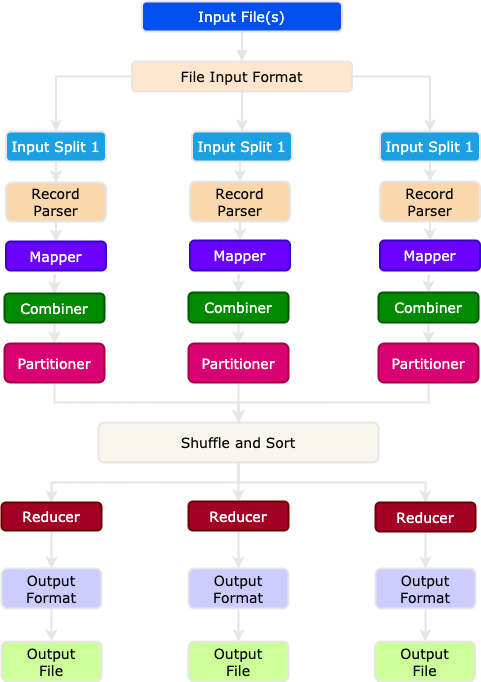
\includegraphics[height=.925\textheight]{./Figures/chapter-02/Map-Reduce.png}
				\caption{Map Reduce Stages } \label{fig:MRSteps}
	\end{figure}			
\end{frame}
%%%%%%%%%%%%%%%%%%%%%%%%%%%%%%%%%%%%%%%%%%%%%%%%%%%%%%
\begin{frame}
	
	\begin{figure}
		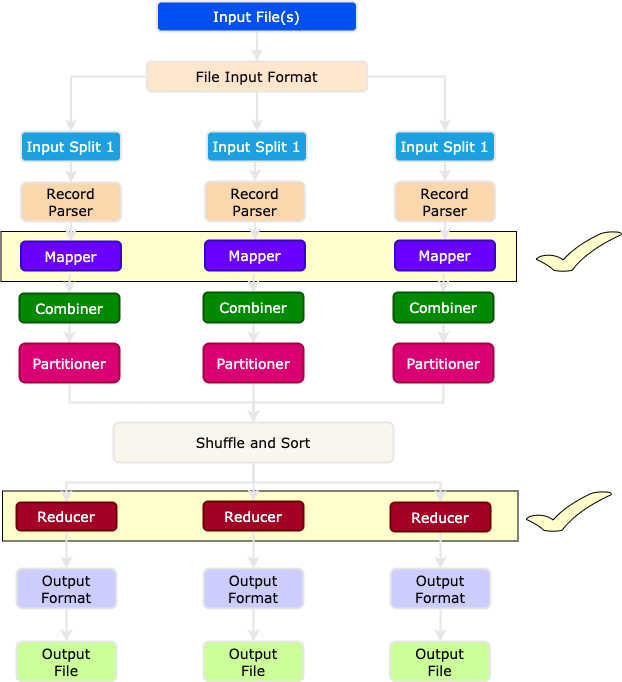
\includegraphics[height=.925\textheight]{./Figures/chapter-02/Map-Reduce_2.png}
		\caption{Map Reduce Stages } \label{fig:MRSteps2}
	\end{figure}			
\end{frame}
%%%%%%%%%%%%%%%%%%%%%%%%%%%%%%%%%%%%%%%%%%%%%%%%%%%%%%
\begin{frame}[c]{ }
	\frametitle{Map Reduce (word count) Deep Dive }
	
	The Map-Reduce consists of three "main" parts
	
	\begin{itemize}  [<+->]
		\item [--] The Driver.
		\item [--] The Mapper.
		\item [--] The Reducer.
		
	\end{itemize}
\end{frame}
%%%%%%%%%%%%%%%%%%%%%%%%%%%%%%%%%%%%%%%%%%%%%%%%%%%%%%
\begin{frame}[c]{ }
	\frametitle{ Hadoop Map Reduce API}
	\centering     
	
	\textcolor{offgreen}{ \large Hadoop Map Reduce API Deep Dive}
\end{frame}
%%%%%%%%%%%%%%%%%%%%%%%%%%%%%%%%%%%%%%%%%%%%%%%%%%%%%%
\begin{frame}[c]{ }
	\frametitle{The Driver }

	\begin{itemize}  [<+->]
		\item [--] The code that runs on the client machine configures the job details by creating an object from the \code{Job}  class, which implements the \code{JobContext} interface.
		\item [--] It submits the job to the cluster.		
		\item [--] It parses job arguments to identify job parameters, for example, input/output directories.. 
		
	\end{itemize}

\end{frame}
%%%%%%%%%%%%%%%%%%%%%%%%%%%%%%%%%%%%%%%%%%%%%%%%%%%%%%
\begin{frame}[c]{ }
	\frametitle{The Driver:  Job Configuration}
	

The \code{Job}  object allows you to set configuration for your \code{Map-Reduce} job:
			\begin{itemize}  [<+->]
				\item [--] You can configure the \code{Mapper} \& the \code{Reducer} classes.
				\item [--] Set the \code{Mapper} input/output key \& value data types.
				\item [--] Set the \code{Reducer} input/output key \& value data types.
	
		
			\end{itemize}		

	
\end{frame}
%%%%%%%%%%%%%%%%%%%%%%%%%%%%%%%%%%%%%%%%%%%%%%%%%%%%%%
\begin{frame}[c]{ }
	\frametitle{The Driver:  Job Configuration}
	
	\begin{itemize}  [<+->]
		\item [--] We can configure file input directory and output.
		\item [--] We configure the output path using \code{FileOutputFormat.setOutputPath()} to specify the reducers' directory to write the output data.
	\end{itemize}		
	
\end{frame}
%%%%%%%%%%%%%%%%%%%%%%%%%%%%%%%%%%%%%%%%%%%%%%%%%%%%%%
\begin{frame}[c]{ }
	\frametitle{The Driver:  Job Configuration}
	
	\begin{itemize}  [<+->]
		\item [--] We configure the input path using \code{FileInputFormat.setInputPaths()}, and by default, it will read all the files in the specified directories and send them to the mappers.
		
		\item [--] We can use \code{Hadoop glob patterns} to read directory patterns, for example, \textit{/warehouse/public/sales*}.
		\item [--] We can call \code{FileInputFormat.addInputPath()} to multiple times by specifying a single file or directory. 
		
	\end{itemize}		
	
	\footnotetext[1]{For more details, please read HTDG. Ch.3 File patterns and PathFilter sections.	} 
\end{frame}
%%%%%%%%%%%%%%%%%%%%%%%%%%%%%%%%%%%%%%%%%%%%%%%%%%%%%%
\begin{frame}[c]{ }
	\frametitle{ Hadoop Map Reduce API}
	\centering     
	
	\textcolor{offgreen}{ \large Please read HTDG. Ch.3 The Java Interface}
\end{frame}
%%%%%%%%%%%%%%%%%%%%%%%%%%%%%%%%%%%%%%%%%%%%%%%%%%%%%%


\begin{frame}[c]{ }
	\frametitle{The Driver:  Job Configuration }
	
		
		\begin{itemize}  [<+->]

			\item [--] You could set driver configurations globally using Hadoop configurations.
			\item [--] Any options not specified in the job configuration will use the Hadoop default values.
			\item [--] We use the \code{Job} object to specify the job name and check its state..
		
			
	\end{itemize}
	
\end{frame}
%%%%%%%%%%%%%%%%%%%%%%%%%%%%%%%%%%%%%%%%%%%%%%%%%%%%%%
\begin{frame}[c]{ }
	\frametitle{The Driver:  Job Configuration }
	

	\begin{itemize}  [<+->]
		
	\item [--] It is optional to set the mapper and reducer classes.
	\item [--] Hadoop uses its default \code{IdentityMapper} and \code{IdentityReducer}.		
		
	\end{itemize}
	
\end{frame}
%%%%%%%%%%%%%%%%%%%%%%%%%%%%%%%%%%%%%%%%%%%%%%%%%%%%%%
\begin{frame}[c]{ }
	\frametitle{The Driver:  Job Configuration }
	
	
	Lunch a Map-Reduce job:
	\begin{itemize}  [<+->]
		
		\item [--] The \code{waitForCompletion()} method in the \code{Job} class launches the job and polls for progress. In addition, it writes the logs and summarizing the Map-Reduce job progress and changes.

	\item [--] When the job completes successfully, the job counters are displayed. Otherwise, the error that caused the job to fail is logged to the console.
		
	\end{itemize}
	
\end{frame}
%%%%%%%%%%%%%%%%%%%%%%%%%%%%%%%%%%%%%%%%%%%%%%%%%%%%%%
\begin{frame}[c]{ }
	\frametitle{InputFormat}
	
	\begin{itemize}  [<+->]
		\item [--] TheThe driver defines the \code{InputFormat}; then the \code{InputFormat} creates a \code{RecordReader"} object that parses the input data into key/value pairs passed to the mapper.
		\item [--] For example: \code{TextInputFormat}:
		\begin{itemize}  [<+->]
			
			\item It is the default.
			\item It creates \code{LineRecordReader} objects.
			\item Key: is the line offest in the file.
			\item Value: is the line which terminated by "\textbackslash n".
		\end{itemize}		
		
		
	\end{itemize}		
	
\end{frame}
%%%%%%%%%%%%%%%%%%%%%%%%%%%%%%%%%%%%%%%%%%%%%%%%%%%%%%
\begin{frame}[c]{ }
	\frametitle{Keys and Values}
	
	\begin{itemize}  [<+->]
		\item [--] Keys and Values in Hadoop are java \code{Objects} not \code{Java primitives types}.
		\item [--] Values are objects which implement \code{Writable}.
		\item [--] Keys are objects which implement \code{WritableComparable}.

		
	\end{itemize}		
	
\end{frame}
%%%%%%%%%%%%%%%%%%%%%%%%%%%%%%%%%%%%%%%%%%%%%%%%%%%%%%
\begin{frame}[c]{ }
	\frametitle{What is Writable?}
	
	\begin{itemize}  [<+->]
		\item [--] \code{Writable} is an interface in Hadoop.
		\item [--] \code{Writables} are used for data type "serialization" in Hadoop to translate/serialize "primitive java data types" to "Hadoop data types", Ex: int to IntWritable and String to Text.
		\item [--] Hadoop uses the \code{Writable} interface for data transfer in the cluster and network.
		
		
	\end{itemize}		
	
\end{frame}
%%%%%%%%%%%%%%%%%%%%%%%%%%%%%%%%%%%%%%%%%%%%%%%%%%%%%%
\begin{frame}[c]{ }
	\frametitle{What is WritableComparable?}
	
	\begin{itemize}  [<+->]
		\item [--] A \code{WritableComparable} is a \code{Writable} which is also \code{Comparable}.
		\item [--] We can compare two \code{WritableComparables} against each other to determine their \textbf{\underline{\textit{order}}}, for example, we could need to compare the order of two Text "Apple vs. Cat or numbers ordering" to understand the ordering mechanism. 
		\item [--] Obviously, the reason we have Keys to be \code{WritableComparable} is that they are passed to the reducer in \underline{\textit{\textbf{sorted order}}}.
		\item [--] Note: All Hadoop implemented types are both \code{Writable} and \code{WritableComparable}.
		
		
	\end{itemize}		
	
\end{frame}
%%%%%%%%%%%%%%%%%%%%%%%%%%%%%%%%%%%%%%%%%%%%%%%%%%%%%%
\begin{frame}[c]{ }
	\frametitle{Map Reduce (word count) Deep Dive }
	
	The Map-Reduce example consists of three main parts
	
	\begin{itemize}  [<+->]
		\item [--] \sout{The Driver}.
		\item [--] The Mapper.

		
	\end{itemize}
\end{frame}
%%%%%%%%%%%%%%%%%%%%%%%%%%%%%%%%%%%%%%%%%%%%%%%%%%%%%%
\begin{frame}[c]{ }
	\frametitle{The Mapper}
		
	\begin{itemize}  [<+->]
		
		\item [--] The mapper class deals with a single input split.
		
		\item [--] All mapper classes must extend the \code{Mapper} base class.

		\item [--] All mapper must specify the key and values for input and output.		
		
		\item [--] All mappers must override the \code{map} method and pass the key, value, and \code{Context}.
		
		\item [--]  The \code{Context} is used to write intermediate data and all information about the job's configurations.
		
	\end{itemize}
	
\end{frame}
%%%%%%%%%%%%%%%%%%%%%%%%%%%%%%%%%%%%%%%%%%%%%%%%%%%%%%
\begin{frame}[c]{ }
	\frametitle{Map Reduce (word count) Deep Dive }
	
	The Map-Reduce example consists of three main parts
	
	\begin{itemize}  [<+->]
		\item [--] \sout{The Driver}.
		\item [--] \sout{The Mapper}.
		\item [--] The Reducer.
		
	\end{itemize}
\end{frame}
%%%%%%%%%%%%%%%%%%%%%%%%%%%%%%%%%%%%%%%%%%%%%%%%%%%%%%
\begin{frame}[c]{ }
	\frametitle{The Reducer}
	
	\begin{itemize}  [<+->]
		
		\item [--] The Reducer receives a Key and an Iterable collection of Writable objects. It also receives a Context object.
		
		\item [--] All reducers classes must extend the  \code{Reducer} base class.
		
		\item [--] All mapper must specify the key and values for intermediate input and final (or intermediate) output.		
		
		\item [--] All reducers must override the "reduce" method and pass the key, \code{Iterable} and "Context".

	\end{itemize}
	
\end{frame}
%%%%%%%%%%%%%%%%%%%%%%%%%%%%%%%%%%%%%%%%%%%%%%%%%%%%%%
\begin{frame}[c]{ }
	\frametitle{ Hadoop Map Reduce API}
	\centering     
	
	\textcolor{offgreen}{ \large Map Reduce Demo}
\end{frame}


%%%%%%%%%%%%%%%%%%%%%%%%%%%%%%%%%%%%%%%%%%%%%%%%%%%%%%
\begin{frame}[c]{ }
	\frametitle{Map Reduce Components }
	
	The Map-Reduce consists of three "main" parts
	
	\begin{itemize}  [<+->]
		\item [--] The Driver.
		\item [--] The Mapper.
		\item [--] The Reducer.
		
	\end{itemize}
\end{frame}

%%%%%%%%%%%%%%%%%%%%%%%%%%%%%%%%%%%%%%%%%%%%%%%%%%%%%%
\begin{frame}
	
	\begin{figure}
		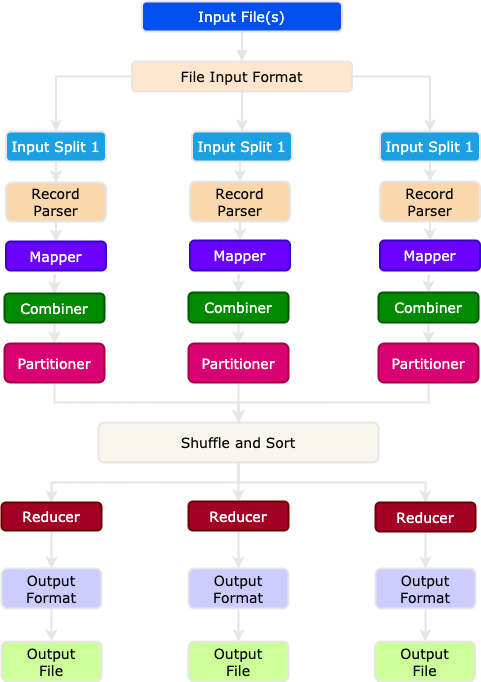
\includegraphics[height=.925\textheight]{./Figures/chapter-02/Map-Reduce.png}
		\caption{Map Reduce Stages } \label{fig:MRSteps}
	\end{figure}			
\end{frame}
%%%%%%%%%%%%%%%%%%%%%%%%%%%%%%%%%%%%%%%%%%%%%%%%%%%%%%
\begin{frame}
	
	\begin{figure}
		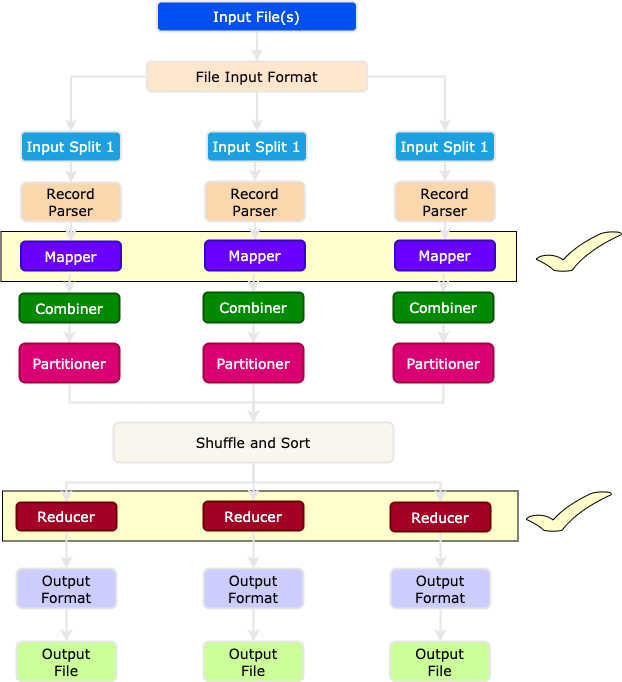
\includegraphics[height=.925\textheight]{./Figures/chapter-02/Map-Reduce_2.png}
		\caption{Map Reduce Stages } \label{fig:MRSteps2}
	\end{figure}			
\end{frame}
%%%%%%%%%%%%%%%%%%%%%%%%%%%%%%%%%%%%%%%%%%%%%%%%%%%%%%
\begin{frame}
	
	\begin{figure}
		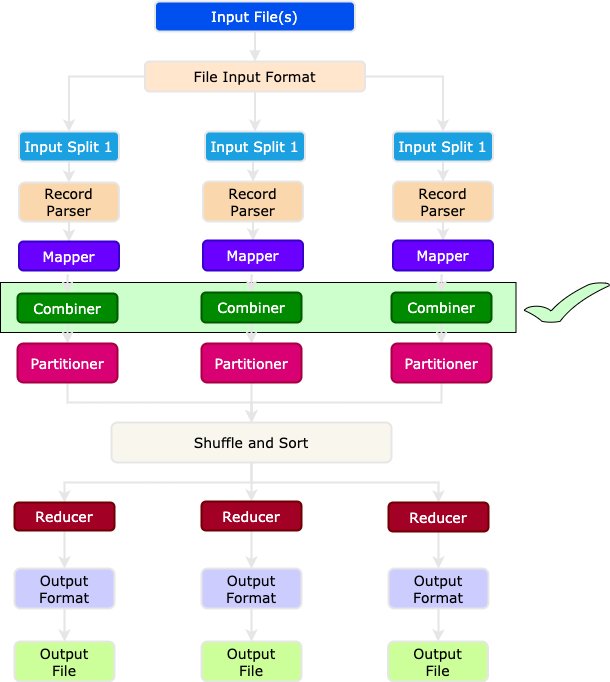
\includegraphics[height=.925\textheight]{./Figures/chapter-02/Map-Reduce-components-combiner.png}
		\caption{Map Reduce Stages } \label{fig:MRSteps2}
	\end{figure}			
\end{frame}

%%%%%%%%%%%%%%%%%%%%%%%%%%%%%%%%%%%%%%%%%%%%%%%%%%%%%%
\begin{frame}[c]{ }
	\frametitle{ The Combiners}
	\centering     
	
	\textcolor{offgreen}{ \large Increase The Map-Reduce Processing Using The Combiners}
\end{frame}
%%%%%%%%%%%%%%%%%%%%%%%%%%%%%%%%%%%%%%%%%%%%%%%%%%%%%%
\begin{frame}
	
	\begin{figure}
		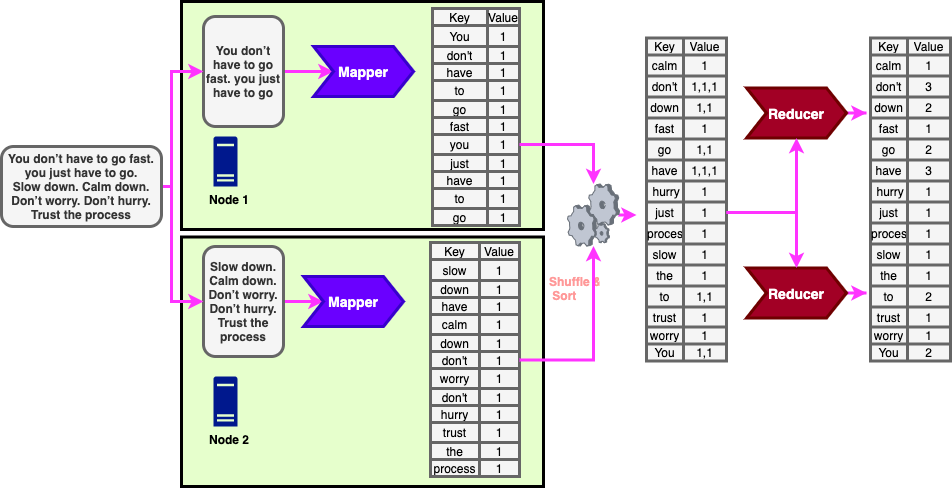
\includegraphics[height=.85\textheight]{./Figures/chapter-02/map-reduce-combiner-ex-1.png}
		\caption{Map Reduce Without Combiner } \label{fig:MRCombiner1}
	\end{figure}			
\end{frame}
%%%%%%%%%%%%%%%%%%%%%%%%%%%%%%%%%%%%%%%%%%%%%%%%%%%%%%
\begin{frame}
	
	\begin{figure}
		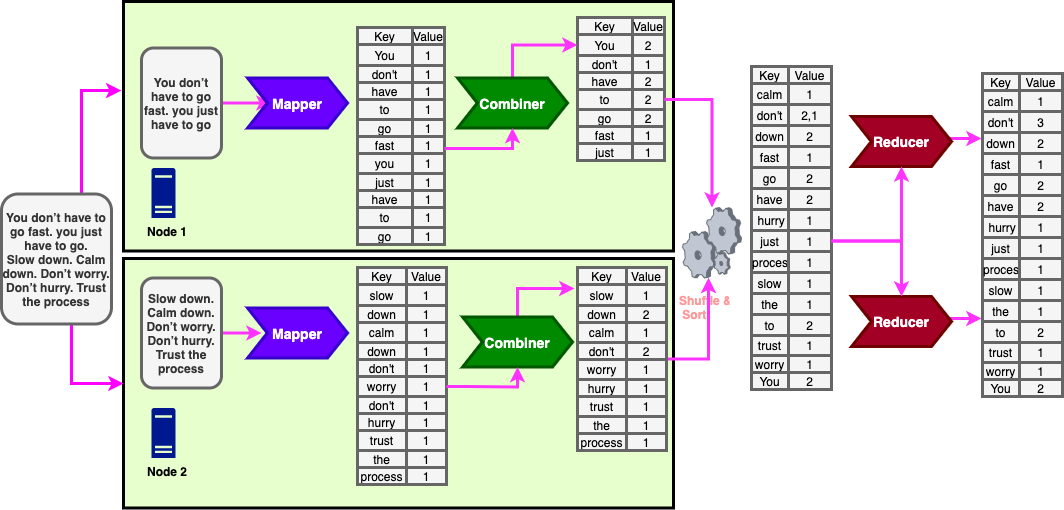
\includegraphics[height=.85\textheight]{./Figures/chapter-02/map-reduce-combiner-ex-2.png}
		\caption{Map Reduce Without Combiner } \label{fig:MRCombiner2}
	\end{figure}			
\end{frame}


%%%%%%%%%%%%%%%%%%%%%%%%%%%%%%%%%%%%%%%%%%%%%%%%%%%%%%%
%\subsection{Further Readings and Assignment}
%
%%%%%%%%%%%%%%%%%%%%%%%%%%%%%%%%%%%%%%%%%%%%%%%%%%%%%%%%%%%%%%%%%%%%%%%%%%%%
%%%% Local Variables:
%%%% mode: latex
%%%% TeX-master: "../main"
%% !TeX root = ../main.tex
%%%% TeX-engine: xetex
%%%% End:
% use no footline.
\begin{frame}[plain, noframenumbering]{Outline}
	\tableofcontents
\end{frame}
%%%%%%%%%%%%%%%%%%%%%%%%%%%%%%%%%%%%%%%%%%%%%%%%%%%%%%
\section{Hive}



\begin{frame}
\frametitle{Chapter Objectives}

\begin{itemize}
	\item<1-> Query data lakes/HDFS using Hive. \pause
	\item<2-> Introduction to Hive \pause
	\item<3-> Comparing Hive to Traditional databases.
	\item<4-> Hive Components and Architecture. \pause
	\item<5-> Relational Data Analysis with Hive. \pause
	\item<6-> Hive Data Management. \pause
	\item<7-> Hive Optimization. \pause
\end{itemize}

\end{frame}

%%%%%%%%%%%%%%%%%%%%%%%%%%%%%%%%%%%%%%%%%%%%%%%%%%%%%%
\subsection{Query data lakes/HDFS using Hive}
\begin{frame}
	\frametitle{\subsecname}
	\begin{itemize} 
		\item Data lakes and HDFS store vast amounts of petabyte-scale data.
		\item Data analysts require efficient ways to query this data without delving into intricate Map-Reduce programming.
		\item SQL is a commonly used language for data manipulation, embraced by data analysts, developers, and business users worldwide.
		\item Hive, one of the early tools in this field, simplifies data analysis on big data by offering SQL-like querying capabilities for data lakes and HDFS.
		\item There are other tools like Trino/Presto, Snowflake, and Databricks that can be faster for data lake queries, which we will discuss later.
	\end{itemize}
	\end{frame}
%%%%%%%%%%%%%%%%%%%%%%%%%%%%%%%%%%%%%%%%%%%%%%%%%%%%%%

\subsection{Introduction to hive}
\begin{frame}
\frametitle{\subsecname}
\begin{itemize} 
	\item Apache Hive is a powerful data warehousing and SQL-like query language tool within the Hadoop ecosystem.
	\item It was developed by Facebook and later contributed to the Apache Software Foundation, making it an open-source project.
	\item Apache Hive had its initial release on October 1, 2010.
	\item Hive provides a user-friendly interface to work with and analyze large datasets stored in Hadoop Distributed File System (HDFS) or other compatible storage systems.
	\item With its SQL-like language called HiveQL, users can write queries to extract, transform, and analyze data, making it accessible to a wide range of data professionals
	\item Apache Hive bridges the gap between the world of big data and traditional relational databases, making it a valuable tool for data engineers, analysts, and data scientists.

\end{itemize}
\end{frame}

%%%%%%%%%%%%%%%%%%%%%%%%%%%%%%%%%%%%%%%%%%%%%%%%%%%%%%


\subsubsection{Overview of Apache Hive}
\begin{frame}
\frametitle{Overview of Apache Hive}
\begin{itemize} 
	\item Apache Hive is a high-level data warehousing and SQL-like query language tool built on top of MapReduce.
	\item It acts as an abstraction layer, allowing users to work with large datasets stored in Hadoop Distributed File System (HDFS) without needing to write complex MapReduce jobs themselves.
	\item Under the hood, Hive generates MapReduce jobs that are executed on the Hadoop cluster. This means it leverages the distributed processing capabilities of Hadoop for scalability and parallel processing.
	\item Hive has evolved beyond MapReduce to support other execution engines, such as Tez and Spark, which can enhance performance and usability. This will be discussed later.

\end{itemize}
\end{frame}

%%%%%%%%%%%%%%%%%%%%%%%%%%%%%%%%%%%%%%%%%%%%%%%%%%%%%%

\subsubsection{Abstract Components of Apache Hive}

\begin{frame}{Abstract Components of Apache Hive}
	\begin{itemize}
		\item Hive Clients.
		\item Hive Services.
		\item Hive Storage and Computing.
	\end{itemize}
	\end{frame}
	
\begin{frame}{Abstract Components of Apache Hive}
	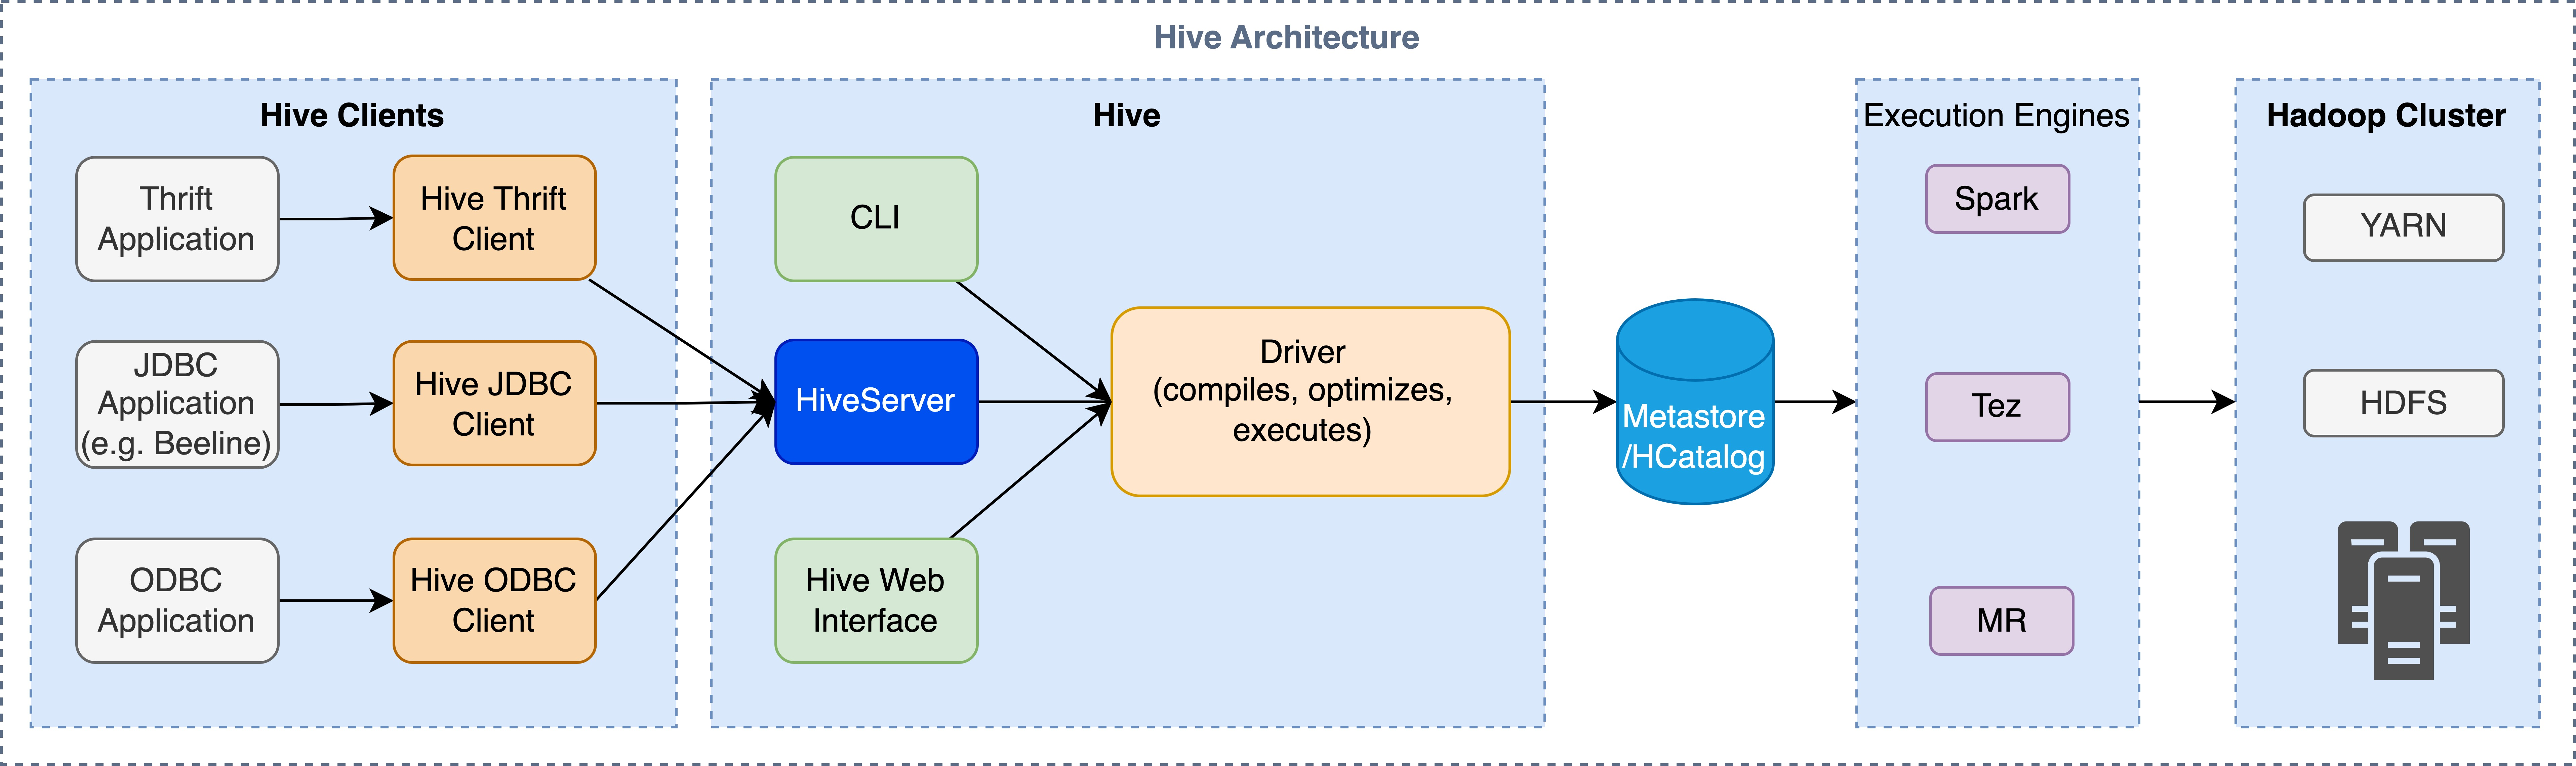
\includegraphics[width=\linewidth,height=.8\textheight]{./Figures/chapter-03/Hive_Architecture.jpg}
\end{frame}
	

%%%%%%%%%%%%%%%%%%%%%%%%%%%%%%%%%%%%%%%%%%%%%%%%%%%%%%
\begin{frame}
\frametitle{Hive Clients}
	\framesubtitle{Connecting with Hive}
	
	\begin{itemize}
	  \item Hive provides various drivers for seamless communication with different types of applications.
	  \item For Thrift-based applications, Hive offers the Thrift client for effective communication.
	  \item If you are working with Java-related applications, Hive provides JDBC drivers for smooth integration.
	  \item Additionally, for other types of applications, Hive offers ODBC drivers, ensuring versatility.
	  \item These clients and drivers serve as intermediaries, connecting your applications with Hive Server in the Hive services.
	\end{itemize}
	
	\end{frame}
%%%%%%%%%%%%%%%%%%%%%%%%%%%%%%%%%%%%%%%%%%%%%%%%%%%%%%
\begin{frame}
	\frametitle{Hive Services}
	\framesubtitle{Client Interactions}
	
	\begin{itemize}
	  \item Hive Services act as the intermediaries for client interactions with Hive.
	  \item When clients need to perform query-related operations in Hive, they communicate through Hive Services.
	  \item The Command Line Interface (CLI) serves as a Hive service for Data Definition Language (DDL) operations.
	  \item All drivers, including JDBC, ODBC, and other client-specific applications, communicate with Hive Server and the primary driver within Hive Services.
	  \item The main driver in Hive Services processes requests from various applications, directing them to the metastore and data systems for further processing.
	\end{itemize}
	
	\end{frame}
%%%%%%%%%%%%%%%%%%%%%%%%%%%%%%%%%%%%%%%%%%%%%%%%%%%%%%

	\begin{frame}
		\frametitle{Hive Services | CLI (Continued)}
		\framesubtitle{Hive CLI Challenges}
		
		\begin{itemize}
		  \item Hive Command Line Interface (CLI)
		  	\begin{itemize}
				\item  The CLI is the most common way to access Hive.
				\item  Its design can make it challenging to use programmatically.
				\item  It is a fat client, requiring a local copy of all Hive components and configurations.
				\item  It needs a copy of a Hadoop client and its configuration.
				\item  The CLI functions as an HDFS client, a MapReduce client, and a JDBC client (for accessing the metastore).
				\item  Even with the correct client installation, ensuring all necessary network access can be complex, especially across subnets or datacenters.
			\end{itemize}
		\end{itemize}
		
		\end{frame}
	%%%%%%%%%%%%%%%%%%%%%%%%%%%%%%%%%%%%%%%%%%%%%%%%%%%%%%

\begin{frame}{Hive Services | HiveServer2 (Continued)}
	\begin{itemize}
		\item \textbf{HiveServer2}: HiveServer2 is a service that allows clients to submit HiveQL queries programmatically. It provides a remote interface for running Hive queries and managing sessions.
		\item \textbf{JDBC and ODBC}: Hive supports JDBC (Java Database Connectivity) and ODBC (Open Database Connectivity) protocols, enabling users to connect to Hive using popular programming languages and tools.
		\item \textbf{Thrift Service}: Hive uses the Apache Thrift framework to provide a cross-language service interface. This enables communication between clients and the Hive server.
		\item \textbf{Sessions}: When clients connect to HiveServer2, sessions are established to manage their interactions. Sessions help keep track of query state and context.
	\end{itemize}
\end{frame}
%%%%%%%%%%%%%%%%%%%%%%%%%%%%%%%%%%%%%%%%%%%%%%%%%%%%%%
\begin{frame}
	\frametitle{Hive Services | HiveServer2 (Continued)}
	\framesubtitle{Introduction to HiveServer2}
	
	\begin{itemize}
	  \item Hive provided a SQL abstraction layer for MapReduce.
	  \item Limitations existed, especially regarding ODBC and JDBC client connections.
	  \item Open source community introduced Hive Server to address these issues.
	  \item Hive Server enabled ODBC connections, enhancing compatibility with various applications.
	\end{itemize}
	
	\end{frame}
%%%%%%%%%%%%%%%%%%%%%%%%%%%%%%%%%%%%%%%%%%%%%%%%%%%%%%
	
	\begin{frame}
	\frametitle{Hive Services | HiveServer2 (Continued)}
	\framesubtitle{Enter Hive Server}
	
	\begin{itemize}
	  \item Hive Server was introduced to overcome limitations.
	  \item Allowed clients to access the metastore using ODBC connections.
	  \item Facilitated integration with applications like Toad, or SQuirreL.
	\end{itemize}
	
	\end{frame}
%%%%%%%%%%%%%%%%%%%%%%%%%%%%%%%%%%%%%%%%%%%%%%%%%%%%%%
	
	\begin{frame}
	\frametitle{Hive Services | HiveServer2 (Continued)}
	\framesubtitle{Challenges with Hive Server}
	
	\begin{itemize}
	  \item While a significant improvement, Hive Server had its limitations:
	  \begin{itemize}
		\item User concurrency restrictions.
		\item Security integration with LDAP posed challenges.
	  \end{itemize}
	\end{itemize}
	
	\end{frame}
%%%%%%%%%%%%%%%%%%%%%%%%%%%%%%%%%%%%%%%%%%%%%%%%%%%%%%
	
	\begin{frame}
	\frametitle{Hive Services | HiveServer2 (Continued)}
	\framesubtitle{Introducing HiveServer2}
	
	\begin{itemize}
	  \item HiveServer2 was designed to overcome Hive Server limitations.
	  \item Built on a Thrift Service architecture.
	  \item Comprises multiple sessions with drivers, compilers, and executors.
	  \item The metastore remains a crucial component, ensuring seamless data management.
	\end{itemize}
	
	\end{frame}
%%%%%%%%%%%%%%%%%%%%%%%%%%%%%%%%%%%%%%%%%%%%%%%%%%%%%%
	
	\begin{frame}
	\frametitle{Hive Services | HiveServer2 (Continued)}
	\framesubtitle{Enhanced Security with HiveServer2}
	
	\begin{itemize}
	  \item HiveServer2 provides enhanced security features.
	  \item Supports various authentication methods, including:
	  \begin{itemize}
		\item Kerberos
		\item Custom authentication
		\item Pass-through LDAP authentication
	  \end{itemize}
	  \item These methods ensure secure client connections.
	\end{itemize}
	
	\end{frame}
%%%%%%%%%%%%%%%%%%%%%%%%%%%%%%%%%%%%%%%%%%%%%%%%%%%%%%
	
	\begin{frame}
	\frametitle{Hive Services | HiveServer2 (Continued)}
	\framesubtitle{Flexible Connection Modes}
	
	\begin{itemize}
	  \item HiveServer2 offers flexibility in connection modes.
	  \item All connection components—JDBC, ODBC, and Beeline—can use any supported authentication method.
	  \item Additionally, HiveServer2 can operate in either HTTP mode or TCP (Binary) mode, catering to diverse connectivity needs.
	\end{itemize}
	
	\end{frame}	
%%%%%%%%%%%%%%%%%%%%%%%%%%%%%%%%%%%%%%%%%%%%%%%%%%%%%%	
\begin{frame}

\frametitle{Hive Services | Hive Driver}
	\framesubtitle{Key Components}
	
	\begin{itemize}
	  \item The Hive Driver is a critical component responsible for query execution.
	  \item It consists of several key components:
		\begin{itemize}
		  \item Query Compiler.
		  \item Optimizer.
		  \item Execution
		\end{itemize}
	  \item Together, these components ensure efficient and effective query processing in Hive.
	\end{itemize}
	
	\end{frame}
%%%%%%%%%%%%%%%%%%%%%%%%%%%%%%%%%%%%%%%%%%%%%%%%%%%%%%
\begin{frame}{Hive Services | Hive Driver (Continued)}
	\begin{itemize}
	\item Query Compiler
		\begin{itemize}
			\item The Query Compiler takes HiveQL queries and translates them into executable jobs.
			\item It's responsible for the logical and physical query planning, ensuring that the queries are optimized for efficient execution.
		\end{itemize}
\end{itemize}
\end{frame}
%%%%%%%%%%%%%%%%%%%%%%%%%%%%%%%%%%%%%%%%%%%%%%%%%%%%%%
\begin{frame}{Hive Services | Hive Driver (Continued)}
\begin{itemize}
\item Query Optimizer	
	\begin{itemize}
		\item It applies optimization techniques, including predicate pushdown and join optimization, to enhance query performance.
		\item This ensures that queries are executed as efficiently as possible.
	\end{itemize}
\end{itemize}
\end{frame}
%%%%%%%%%%%%%%%%%%%%%%%%%%%%%%%%%%%%%%%%%%%%%%%%%%%%%%
\begin{frame}{Hive Services | Hive Driver (Continued)}
\begin{itemize}
    \item The Execution Engine is responsible for the actual execution of queries.
    \item It encompasses several key tasks, including:
    \begin{itemize}
        \item \textbf{Plan Execution}: It executes the query plan generated by the Query Compiler.
        \item \textbf{Job(s) Generation}: Depending on the chosen execution engine (e.g., MapReduce), it generates the necessary jobs to process data in parallel.
        \item \textbf{Submission to Hadoop}: It submits these jobs to the Hadoop cluster or other compatible compute environments for execution.
        \item \textbf{Progress Monitoring}: It continuously monitors the progress of the query execution, providing insights into job completion and overall performance.
    \end{itemize}
\end{itemize}
\end{frame}


%%%%%%%%%%%%%%%%%%%%%%%%%%%%%%%%%%%%%%%%%%%%%%%%%%%%%%

\begin{frame}{Metadata Store (e.g., MySQL)}
	\begin{itemize}
		\item The Metadata Store is a relational database, such as MySQL, that stores critical information about tables, columns, partitions, and their relationships.
		\item This database acts as a catalog, enabling Hive to understand the data's structure and schema.
	\end{itemize}
\end{frame}
%%%%%%%%%%%%%%%%%%%%%%%%%%%%%%%%%%%%%%%%%%%%%%%%%%%%%%

\begin{frame}{Data Storage}
\begin{itemize}
    \item Hive operates on data stored in HDFS or compatible storage systems.
    \item Instead of transforming the data, it interprets it using a schema on read approach.
    \item This allows users to work with data without the need for extensive data preparation.
\end{itemize}
\end{frame}
%%%%%%%%%%%%%%%%%%%%%%%%%%%%%%%%%%%%%%%%%%%%%%%%%%%%%%
\subsubsection{Job Execution Flow in Hive}
\begin{frame}{Job Execution Flow in Hive}
	\begin{itemize}
		\item Receive SQL Query.
		\begin{itemize}
			\item Parse HiveQL.
			\item Make optimization.
			\item Plan execution.
			\item Submit job(s) to the cluster.
			\item Monitor the progress.
			\item Process the data in MapReduce or Spark.
			\item Store the data in HDFS.
		\end{itemize}
	\end{itemize}
	\end{frame}
%%%%%%%%%%%%%%%%%%%%%%%%%%%%%%%%%%%%%%%%%%%%%%%%%%%%%%
\subsubsection{Hive Schema and Data Storage}
\begin{frame}{Hive Schema and Data Storage}
	\begin{itemize}
		\item Hive queries operate on tables, similar to RDBMS.
		\begin{itemize}
			\item A table corresponds to a directory in storage (HDFS, S3, GCS, or Azure).
			\item Each table comprises one or more files.
			\item Every table is associated with a specific file format.
			\item Hive stores table structure and location in the metadata store (RDBMS).
			\item Hive supports various file formats, such as Parquet, ORC, and Text.
		\end{itemize}
	\end{itemize}
\end{frame}

\begin{frame}{Hive Schema and Data Storage (Continued)}
	\begin{itemize}
		\item Hive queries reference the metastore to access table location and structure.
		\item While queries interact with the file system, metadata is stored in the RDBMS.
	\end{itemize}
\end{frame}

%%%%%%%%%%%%%%%%%%%%%%%%%%%%%%%%%%%%%%%%%%%%%%%%%%%%%%

\subsection{Performance Tuning}
%%%%%%%%%%%%%%%%%%%%%%%%%%%%%%%%%%%%%%%%%%%%%%%%%%%%%%
\subsubsection{Query Execution Plan}
\begin{frame}
	\frametitle{Query Execution Plan}
	\framesubtitle{Overview}
	
	\begin{itemize}
	  \item The Hive driver is responsible for translating SQL statements into an execution plan for the target execution engine.
	  \item The process involves several key steps:
		\begin{enumerate}
		  \item The parser parses the SQL statement and generates an Abstract Syntax Tree (AST) representing logical operations like SELECTs, JOINs, UNIONs, groupings, and more.
		  \item The planner retrieves table metadata from the Hive Metastore, including HDFS file locations, storage formats, row counts, etc.
		  \item The query optimizer utilizes the AST and table metadata to produce a physical operation tree known as the execution plan, defining the physical operations needed to retrieve data, such as nested loop joins, sort-merge joins, hash joins, index joins, and more.
		\end{enumerate}

	\end{itemize}
	
	\end{frame}
	
	\begin{frame}
	\frametitle{Query Execution Plan}
	\framesubtitle{Impact on Performance}
	
	\begin{itemize}
	\item The execution plan determines the tasks executed on the Hadoop cluster and significantly impacts performance in data analytics systems like Hive.
	  \item The execution plan generated by the query optimizer has a substantial impact on performance.
	  \item Differences in the execution plan can result in significant variations in execution time, ranging from seconds to hours.
	  \item An optimal execution plan is crucial for efficient query processing in Hive.
	\end{itemize}
	
	\end{frame}
	
	\begin{frame}
	\frametitle{Query Execution Plan}
	\framesubtitle{Cost-Based Optimization (CBO)}
	
	\begin{itemize}
	  \item The Cost-Based Optimization (CBO) plays a pivotal role in enhancing the execution plan.
	  \item CBO leverages table statistics to make informed decisions regarding the performance costs associated with each potential execution plan.
	  \item This intelligent optimization ensures that the Hive driver produces an optimal execution plan, improving query performance.
	\end{itemize}
	
	\end{frame}
\subsubsection{Cost-Based Optimization}
\subsection{Further Readings and Assignment}


%%%%%%%%%%%%%%%%%%%%%%%%%%%%%%%%%%%%%%%%%%%%%%%%%%%%%%%%%%%%%%%%%%%%%%%%%%%
%%% Local Variables:
%%% mode: latex
%%% TeX-master: "../main"
% !TeX root = ../main.tex
%%% TeX-engine: xetex
%%% End:
%    \include{Ch04-Spark/FN-Scala}
%    \include{Ch04-Spark/Spark}
%    \include{Ch05-BigData-Applications/Applications}
%    \include{Ch06-Massaging-Systems/Massaging-Systems}
%    \include{Ch07-DataOrchestration/Orchestration}
%    \include{Ch08-NoSqlDB/NoSql}
%    \include{Ch09-Elastic/Elastic}
%    \include{Ch10-Architecture/Architecture}
%    \include{Appendix/Appendix}
%%%%%%%%%%%%%%%%%%%%%%%%%%%%%%%%%%%%%%%%%%%%%%%%%%%%%%

\begin{frame}[c]{ }
    \centering     
   
    \textcolor{offgreen}{ \large Thank you for watching!}
\end{frame}


\begin{frame}[c]{ }
    \centering 
    \textcolor{offyellow}{\large See you in the next video \Smiley{}}
\end{frame}
    %%%%%%%%%%%%%%%%%%%%%%%%%%%%%%%%%%%%%%%%%%%%%%%%%%%%%%%%%%%%%%%%%%%%%%%%%%%%%%%%%%%%%%%
\end{document}

%%% Local Variables:
%%% mode: latex
%%% TeX-master: t
%%% TeX-engine: xetex
%%% End:
